%%%% fs-run-time-graph  Graph and its partitioning

\label {fs-graph}

In our model, the stream between front and barrier is handled by a directed data flow graph. Each node of the graph contains single operation, also called job or procedure, which can have multiple inputs and outputs. Edges show the order of these operations. The data items are processed one-by-one in a "streaming" manner.

Notably, despite the fact that commonly dataflow graphs assumed to be acyclic (DAGs) 
~\cite{Zaharia:2016:ASU:3013530.2934664, Carbone:2017:SMA:3137765.3137777},
our model does not have this restriction. Moreover, as we show further in this section, there are cases when cycles are required, e.g. for MapReduce-based algorithms. 

\subsection{Physical deployment and partitioning}

Each computational unit in our distributed runtime runs process called {\it worker}, and each worker executes complete data flow graph. Every worker is assigned by an integer interval. Intervals are not intersected and cover the range of 32-bit signed integer.

Each input of each operation is assigned by user-provided hash function called {\it balancing function}. This function is applied to the payload of data items and determines partitioning. More precisely, its value is computed each time before the next operation. After that, corresponding data item is sent to the worker, which is responsible for the computed value. Therefore, load balancing explicitly depends on the balancing functions of the operations. The balancing functions are the part of business logic, because optimal balancing requires the knowledge of payload distribution.

Figure~\ref{logical-graph-figure} shows the example of data flow graph. Possible partitioning of this graph on two nodes is shown on the figure~\ref{physical-graph-figure}.

\begin{figure}[htbp]
  \centering
  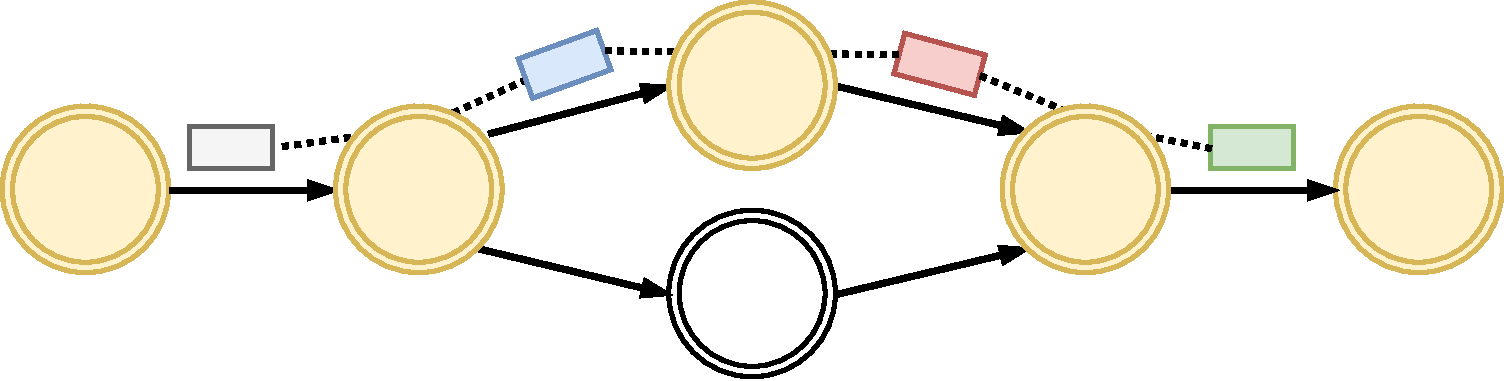
\includegraphics[width=0.48\textwidth]{pics/logical-graph}
  \caption{The example of data flow graph}
  \label {logical-graph-figure}
\end{figure}

\begin{figure}[htbp]
  \centering
  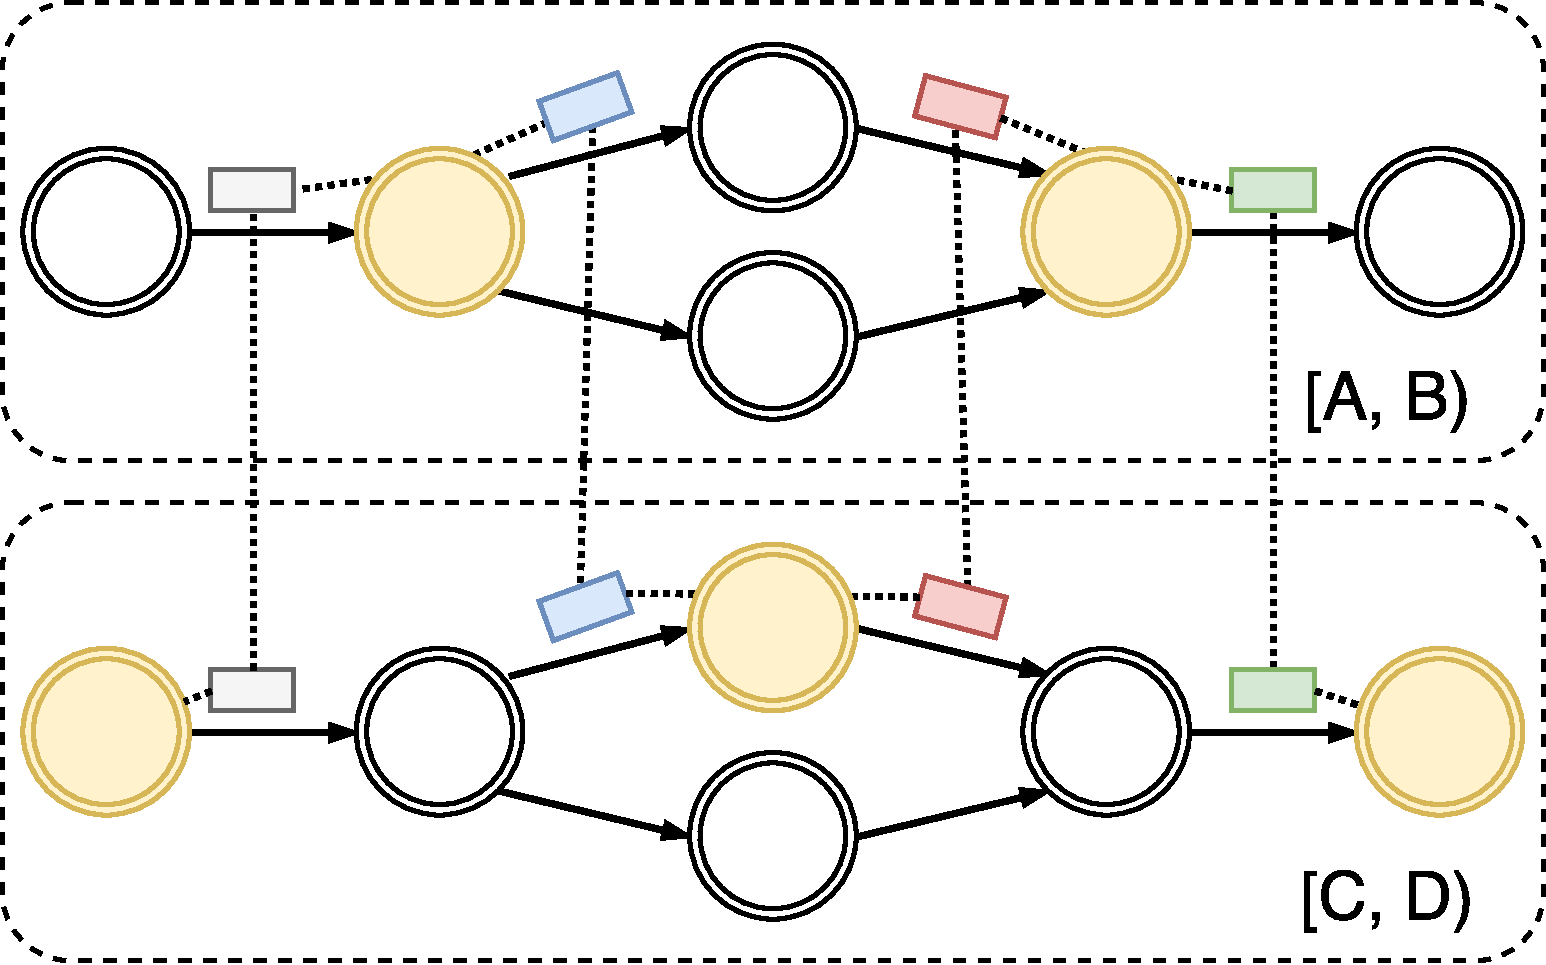
\includegraphics[width=0.48\textwidth]{pics/physical-graph}
  \caption{Possible partitioning of the data flow graph}
  \label {physical-graph-figure}
\end{figure}
